% answers.tex —— 2008 年·普通高等学校招生考试·四川卷·理科 · 参考答案与详细解析片段
% 由 tools/generate_projects.py 依来源总账自 2008/2008_数学真题_四川理_试题.md + 2008/2008_数学真题_四川理_解析正文.md + 2008/2008_数学真题_四川理_答案要点.md 生成，勿手改（改源 MD 后重跑）


\begin{gktip}
固定候选 PDF 仅含题面、无答案与解析；以下为非官方编者独立推导。
\end{gktip}

\begin{answer}
\gksolhead{1}{}

\textbf{题目}：

设集合 $U=\{1,2,3,4,5\}$，$A=\{1,2,3\}$，$B=\{2,3,4\}$，则 $\complement_U(A\cap B)=$（　）

（A）$\{2,3\}$

（B）$\{1,4,5\}$

（C）$\{4,5\}$

（D）$\{1,5\}$

\Needspace{4\baselineskip}
\textbf{解析}

$A\cap B=\{2,3\}$，故 $\complement_U(A\cap B)=\{1,4,5\}$。

\gkanswer{答案：B。}

\end{answer}
\begin{answer}
\gksolhead{2}{}

\textbf{题目}：

复数 $2\mathrm i(1+\mathrm i)^2=$（　）

（A）$-4$

（B）$4$

（C）$-4\mathrm i$

（D）$4\mathrm i$

\Needspace{4\baselineskip}
\textbf{解析}

$2\mathrm i(1+\mathrm i)^2=2\mathrm i\cdot2\mathrm i=4\mathrm i^2=-4$。

\gkanswer{答案：A。}

\end{answer}
\begin{answer}
\gksolhead{3}{}

\textbf{题目}：

$(\tan x+\cot x)\cos^2x=$（　）

（A）$\tan x$

（B）$\sin x$

（C）$\cos x$

（D）$\cot x$

\Needspace{4\baselineskip}
\textbf{解析}

$(\tan x+\cot x)\cos^2x=\dfrac{\sin^2x+\cos^2x}{\sin x\cos x}\cos^2x=\dfrac{\cos x}{\sin x}=\cot x$。

\gkanswer{答案：D。}

\end{answer}
\begin{answer}
\gksolhead{4}{}

\textbf{题目}：

直线 $y=3x$ 绕原点逆时针旋转 $90^\circ$，再向右平移 $1$ 个单位，所得到的直线为（　）

（A）$y=-\dfrac13x+\dfrac13$

（B）$y=-\dfrac13x+1$

（C）$y=3x-3$

（D）$y=\dfrac13x+1$

\Needspace{4\baselineskip}
\textbf{解析}

旋转 $90^\circ$ 得 $y=-\dfrac13x$，再右移 $1$ 个单位得 $y=-\dfrac13(x-1)=-\dfrac13x+\dfrac13$。

\gkanswer{答案：A。}

\end{answer}
\begin{answer}
\gksolhead{5}{}

\textbf{题目}：

若 $0\leqslant\alpha\leqslant2\pi$，$\sin\alpha>\sqrt3\cos\alpha$，则 $\alpha$ 的取值范围是（　）

（A）$\left(\dfrac{\pi}3,\dfrac{\pi}2\right)$

（B）$\left(\dfrac{\pi}3,\pi\right)$

（C）$\left(\dfrac{\pi}3,\dfrac{4\pi}3\right)$

（D）$\left(\dfrac{\pi}3,\dfrac{3\pi}2\right)$

\Needspace{4\baselineskip}
\textbf{解析}

$\sin\alpha>\sqrt3\cos\alpha$：当 $\cos\alpha>0$ 时等价于 $\tan\alpha>\sqrt3$，得 $\alpha\in\left(\dfrac{\pi}3,\dfrac{\pi}2\right)$；当 $\cos\alpha<0$ 时左正右负，恒成立，得 $\alpha\in\left(\dfrac{\pi}2,\pi\right)$；$\cos\alpha=0$ 时 $\sin\alpha=1>0$ 也成立。合并得 $\alpha\in\left(\dfrac{\pi}3,\pi\right)$。

\gkanswer{答案：B。}

\end{answer}
\begin{answer}
\gksolhead{6}{}

\textbf{题目}：

从甲、乙等 $10$ 个同学中挑选 $4$ 名参加某项公益活动，要求甲、乙中至少有 $1$ 人参加，则不同的挑选方法共有（　）

（A）$70$ 种

（B）$112$ 种

（C）$140$ 种

（D）$168$ 种

\Needspace{4\baselineskip}
\textbf{解析}

$\mathrm C_{10}^4-\mathrm C_8^4=210-70=140$。

\gkanswer{答案：C。}

\end{answer}
\begin{answer}
\gksolhead{7}{}

\textbf{题目}：

已知等比数列 $\{a_n\}$ 中 $a_2=1$，则其前 $3$ 项的和 $S_3$ 的取值范围是（　）

（A）$(-\infty,-1]$

（B）$(-\infty,0)\cup(1,+\infty)$

（C）$[3,+\infty)$

（D）$(-\infty,-1]\cup[3,+\infty)$

\Needspace{4\baselineskip}
\textbf{解析}

\Needspace{5\baselineskip}
设公比 $q$（$q\neq0$），$a_2=1$ 给 $a_1=\dfrac1q$，$a_3=q$，故

\nopagebreak[4]
\[S_3=q+\frac1q+1.\]

$q>0$ 时 $q+\dfrac1q\geqslant2$，$S_3\geqslant3$（$q=1$ 取等）；$q<0$ 时 $q+\dfrac1q\leqslant-2$，$S_3\leqslant-1$（$q=-1$ 取等）。故 $S_3\in(-\infty,-1]\cup[3,+\infty)$。

\gkanswer{答案：D。}

\end{answer}
\begin{answer}
\gksolhead{8}{}

\textbf{题目}：

设 $M$，$N$ 是球心 $O$ 的半径 $OP$ 上的两点，且 $NP=MN=OM$，分别过 $N$，$M$，$O$ 作垂直于 $OP$ 的平面，截球面得三个圆，则这三个圆的面积之比为（　）

（A）$3:5:6$

（B）$3:6:8$

（C）$5:7:9$

（D）$5:8:9$

\Needspace{4\baselineskip}
\textbf{解析}

设球半径 $R$，由 $OM=MN=NP$ 得 $OM=\dfrac R3$、$ON=\dfrac{2R}3$。三个截面圆半径平方依次为 $R^2$（过 $O$）、$R^2-\dfrac{R^2}9=\dfrac89R^2$（过 $M$）、$R^2-\dfrac{4R^2}9=\dfrac59R^2$（过 $N$），故面积比为 $9:8:5$，即 (D) 的 $5:8:9$。

\gkanswer{答案：D。}

\end{answer}
\begin{answer}
\gksolhead{9}{}

\textbf{题目}：

设直线 $l\subset$ 平面 $\alpha$，过平面 $\alpha$ 外一点 $A$ 与 $l$、$\alpha$ 都成 $30^\circ$ 角的直线有且只有（　）

（A）$1$ 条

（B）$2$ 条

（C）$3$ 条

（D）$4$ 条

\Needspace{4\baselineskip}
\textbf{解析}

取 $\alpha$ 为 $xOy$ 平面、$l$ 沿 $x$ 轴。方向向量 $d$ 满足 $|d_z|=\dfrac{|d|}2$（与 $\alpha$ 成 $30^\circ$）与 $|d_x|=\dfrac{\sqrt3|d|}2$（与 $l$ 成 $30^\circ$），故 $d_y=0$，只有 $\left(\dfrac{\sqrt3}2,0,\pm\dfrac12\right)$ 两类方向，即 $2$ 条。

\gkanswer{答案：B。}

\end{answer}
\begin{answer}
\gksolhead{10}{}

\textbf{题目}：

设 $f(x)=\sin(\omega x+\varphi)$，其中 $\omega>0$，则 $f(x)$ 是偶函数的充要条件是（　）

（A）$f(0)=1$

（B）$f(0)=0$

（C）$f'(0)=1$

（D）$f'(0)=0$

\Needspace{4\baselineskip}
\textbf{解析}

$f$ 为偶函数 $\iff$ 对一切 $x$ 有 $\sin(-\omega x+\varphi)=\sin(\omega x+\varphi)$ $\iff$ $\cos\varphi=0$。又 $f'(x)=\omega\cos(\omega x+\varphi)$，$f'(0)=\omega\cos\varphi$，故充要条件为 $f'(0)=0$。

\gkanswer{答案：D。}

\end{answer}
\begin{answer}
\gksolhead{11}{}

\textbf{题目}：

设定义在 $\mathbf R$ 上的函数 $f(x)$ 满足 $f(x)\cdot f(x+2)=13$，若 $f(1)=2$，则 $f(99)=$（　）

（A）$13$

（B）$2$

（C）$\dfrac{13}2$

（D）$\dfrac2{13}$

\Needspace{4\baselineskip}
\textbf{解析}

$f(x+2)=\dfrac{13}{f(x)}$，故 $f(x+4)=f(x)$，周期 $4$，$f(99)=f(3)=\dfrac{13}{f(1)}=\dfrac{13}2$。

\gkanswer{答案：C。}

\end{answer}
\begin{answer}
\gksolhead{12}{}

\textbf{题目}：

已知抛物线 $C:y^2=8x$ 的焦点为 $F$，准线与 $x$ 轴的交点为 $K$，点 $A$ 在 $C$ 上且 $|AK|=\sqrt2|AF|$，则 $\triangle AFK$ 的面积为（　）

（A）$4$

（B）$8$

（C）$16$

（D）$32$

\Needspace{4\baselineskip}
\textbf{解析}

\Needspace{5\baselineskip}
$F(2,0)$，$K(-2,0)$。设 $A(x,y)$，则 $|AF|=x+2$，$|AK|^2=(x+2)^2+y^2=(x+2)^2+8x$。由 $|AK|=\sqrt2|AF|$：

\nopagebreak[4]
\[(x+2)^2+8x=2(x+2)^2\iff 8x=(x+2)^2\iff x=2,\]

故 $y^2=16$，$|y|=4$。$S_{\triangle AFK}=\dfrac12\cdot4\cdot4=8$。

\gkanswer{答案：B。}

\end{answer}
\begin{answer}
\gksolhead{13}{}

\textbf{题目}：

$(1+2x)^3(1-x)^4$ 展开式中 $x^2$ 的系数为\gkblank{}。

\Needspace{4\baselineskip}
\textbf{解析}

$(1+2x)^3(1-x)^4$ 的 $x^2$ 项：$1\cdot6x^2+6x\cdot(-4x)+12x^2\cdot1=(6-24+12)x^2=-6x^2$。

\gkanswer{答案：$-6$。}

\end{answer}
\begin{answer}
\gksolhead{14}{}

\textbf{题目}：

已知直线 $l:x-y+4=0$ 与圆 $C:(x-1)^2+(y-1)^2=2$，则 $C$ 上各点到 $l$ 的距离的最小值为\gkblank{}。

\Needspace{4\baselineskip}
\textbf{解析}

圆心 $(1,1)$ 到 $l$ 的距离 $\dfrac{4}{\sqrt2}=2\sqrt2$，减去半径 $\sqrt2$ 得 $\sqrt2$。

\gkanswer{答案：$\sqrt2$。}

\end{answer}
\begin{answer}
\gksolhead{15}{}

\textbf{题目}：

已知正四棱柱的对角线的长为 $\sqrt6$，且对角线与底面所成角的余弦值为 $\dfrac{\sqrt3}3$，则该正四棱柱的体积等于\gkblank{}。

\Needspace{4\baselineskip}
\textbf{解析}

设底面边长 $a$、高 $h$，则对角线 $\sqrt{2a^2+h^2}=\sqrt6$，且 $\cos\theta=\dfrac{\sqrt2a}{\sqrt{2a^2+h^2}}=\dfrac{\sqrt3}3$，故 $\sqrt2a=\sqrt2$，$a=1$，$h=2$，$V=a^2h=2$。

\gkanswer{答案：$2$。}

\end{answer}
\begin{answer}
\gksolhead{16}{}

\textbf{题目}：

设等差数列 $\{a_n\}$ 的前 $n$ 项和为 $S_n$，若 $S_4\geqslant10$，$S_5\leqslant15$，则 $a_4$ 的最大值为\gkblank{}。

\Needspace{4\baselineskip}
\textbf{解析}

\Needspace{5\baselineskip}
$S_4=4a_1+6d\geqslant10$ 即 $2a_1+3d\geqslant5$；$S_5=5a_1+10d\leqslant15$ 即 $a_1+2d\leqslant3$。两式消去 $a_1$ 得 $d\leqslant1$，于是

\nopagebreak[4]
\[a_4=a_1+3d=(a_1+2d)+d\leqslant3+1=4,\]

当 $a_1=1$、$d=1$ 时取到（此时 $S_4=10$、$S_5=15$）。

\gkanswer{答案：$4$。}

\end{answer}
\begin{answer}
\gksolhead{17}{}

\textbf{题目}：

求函数 $y=7-4\sin x\cos x+4\cos^2x-4\cos^4x$ 的最大值与最小值。

\Needspace{4\baselineskip}
\textbf{解析}

$y=7-2\sin2x+4\cos^2x\sin^2x=7-2\sin2x+\sin^22x=(\sin2x-1)^2+6$，故 $y\in[6,10]$。

\gkanswer{答案：最大值 $10$，最小值 $6$。}

\end{answer}
\begin{answer}
\gksolhead{18}{}

\textbf{题目}：

设进入某商场的每一位顾客购买甲种商品的概率为 $0.5$，购买乙种商品的概率为 $0.6$，且购买甲种商品与购买乙种商品相互独立，各顾客之间购买商品也是相互独立的。

（1）求进入商场的 $1$ 位顾客购买甲、乙两种商品中的一种的概率；

（2）求进入商场的 $1$ 位顾客至少购买甲、乙两种商品中的一种的概率；

（3）记 $\xi$ 表示进入商场的 $3$ 位顾客中至少购买甲、乙两种商品中的一种的人数，求 $\xi$ 的分布列及期望。

\Needspace{4\baselineskip}
\textbf{解析}

（1）只买一种：$0.5\times0.4+0.5\times0.6=0.5$。

（2）$1-0.5\times0.4=0.8$。

\Needspace{5\baselineskip}
（3）每位顾客至少买一种的概率 $p=0.8$，$\xi\sim B(3,0.8)$：

\nopagebreak[4]
\[P(\xi=0)=0.008,\quad P(\xi=1)=0.096,\quad P(\xi=2)=0.384,\quad P(\xi=3)=0.512,\]

故 $E\xi=3\times0.8=2.4$。

\gkanswer{答案：（1）$0.5$；（2）$0.8$；（3）分布列见解析，$E\xi=2.4$。}

\end{answer}
\begin{answer}
\gksolhead{19}{}

\textbf{题目}：

如图，平面 $ABEF\perp$ 平面 $ABCD$，四边形 $ABEF$ 与 $ABCD$ 都是直角梯形，$\angle BAD=\angle FAB=90^\circ$，$BC\parallel\dfrac12AD$，$BE\parallel\dfrac12AF$。

（1）证明：$C$、$D$、$F$、$E$ 四点共面；

（2）设 $AB=BC=BE$，求二面角 $A-ED-B$ 的大小。
\nopagebreak[4]
\begin{center}% 2008 年四川卷理科第 19 题：平面 ABEF ⊥ 平面 ABCD，两个直角梯形 ABEF、ABCD，
%   ∠BAD = ∠FAB = 90°，BC ∥= ½AD，BE ∥= ½AF。
% 来源 PDF：gaokaomath-src/普通高考/2008/2008四川理.pdf
% SHA-256：dd251cfc43d7be2f75e2675f8bd73e8569900c65a53724312a95b1cec79a3a9b
% 原页：2008四川理.pdf 第 1 页（A3 三栏）第 3 栏，书页码 483。
% 重绘依据：与文科卷第 19 题同一几何体（理卷无 G、H），投影 (x,y,z)->(x+0.8y, 0.5y+z)。
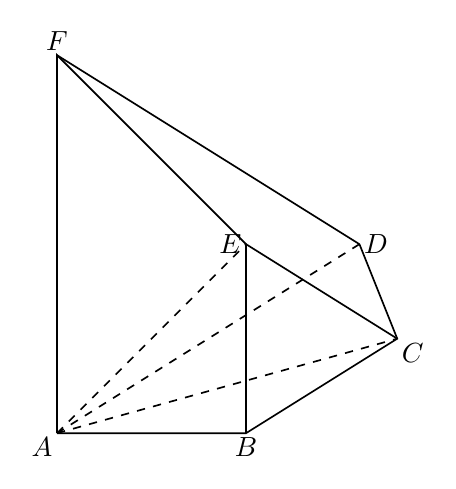
\begin{tikzpicture}[scale=1.2, semithick, every node/.style={inner sep=1.4pt}]
  \coordinate (A) at (0.00,0.00);
  \coordinate (B) at (2.00,0.00);
  \coordinate (C) at (3.60,1.00);
  \coordinate (D) at (3.20,2.00);
  \coordinate (F) at (0.00,4.00);
  \coordinate (E) at (2.00,2.00);

  % 底面 ABCD
  \draw (A) -- (B) -- (C) -- (D);
  \draw[dashed] (D) -- (A);
  \draw[dashed] (A) -- (C);

  % 立面 ABEF
  \draw (A) -- (F) -- (E) -- (B);

  % 侧棱与内部虚线
  \draw (C) -- (E);
  \draw (D) -- (F);
  \draw[dashed] (A) -- (E);

  \node[below left] at (A) {$A$};
  \node[below] at (B) {$B$};
  \node[below right] at (C) {$C$};
  \node[right] at (D) {$D$};
  \node[above] at (F) {$F$};
  \node[left] at (E) {$E$};
\end{tikzpicture}
\end{center}
\nopagebreak[4]
\Needspace{4\baselineskip}
\textbf{解析}

\Needspace{5\baselineskip}
取 $A$ 为原点，$AB$ 为 $x$ 轴、$AD$ 为 $y$ 轴，$AF$ 垂直于底面。设 $AB=BC=BE=2$，则 $AD=AF=4$，

\nopagebreak[4]
\[A(0,0,0),\ B(2,0,0),\ C(2,2,0),\ D(0,4,0),\ E(2,0,2),\ F(0,0,4).\]

（1）$\overrightarrow{CE}=\left(0,-2,\dfrac f2\right)$ 型计算给出 $(\overrightarrow{CE}\times\overrightarrow{CF})\cdot\overrightarrow{CD}=0$（$f=4$），故 $C$、$D$、$F$、$E$ 四点共面。

\Needspace{5\baselineskip}
（2）平面 $AED$ 的法向量 $\overrightarrow{AE}\times\overrightarrow{AD}=(-8,0,8)$，取 $(-1,0,1)$；平面 $BED$ 的法向量 $\overrightarrow{BE}\times\overrightarrow{BD}=(-8,-4,0)$，取 $(2,1,0)$。于是

\nopagebreak[4]
\[\cos\theta=\frac{|(-1)\cdot2+0+0|}{\sqrt2\cdot\sqrt5}=\frac{\sqrt{10}}5,\]

二面角 $A-ED-B$ 为 $\arccos\dfrac{\sqrt{10}}5$。

\gkanswer{答案：（1）证明见解析；（2）$\arccos\dfrac{\sqrt{10}}5$。}

\end{answer}
\begin{answer}
\gksolhead{20}{}

\textbf{题目}：

设数列 $\{a_n\}$ 的前 $n$ 项和为 $S_n$，已知 $ba_n-2^n=(b-1)S_n$。

（1）证明：当 $b=2$ 时，$\{a_n-n\cdot2^{n-1}\}$ 是等比数列；

（2）求 $\{a_n\}$ 的通项公式。

\Needspace{4\baselineskip}
\textbf{解析}

\Needspace{5\baselineskip}
（1）令 $b=2$，则 $2a_n-2^n=S_n$。由 $n=1$ 得 $a_1=2$；由 $a_n=S_n-S_{n-1}$（$n\geqslant2$）得

\nopagebreak[4]
\[2a_n-2^n-(2a_{n-1}-2^{n-1})=a_n\iff a_n=2a_{n-1}+2^{n-1}.\]

\Needspace{5\baselineskip}
记 $c_n=a_n-n\cdot2^{n-1}$，则

\nopagebreak[4]
\[c_n=2a_{n-1}+2^{n-1}-n2^{n-1}=2\left[a_{n-1}-(n-1)2^{n-2}\right]=2c_{n-1},\]

且 $c_1=a_1-1=1\neq0$，故 $\{c_n\}$ 是首项 $1$、公比 $2$ 的等比数列。

\Needspace{5\baselineskip}
（2）由（1）$c_n=2^{n-1}$，故

\nopagebreak[4]
\[a_n=n\cdot2^{n-1}+2^{n-1}=(n+1)2^{n-1}.\]

（一般 $b$：$a_1=\dfrac2b$，递推 $a_n=ba_{n-1}+2^{n-1}$；$b=1$ 时 $a_n=2^n$，$b\neq0,1,2$ 时 $a_n=\dfrac{2^n+4(1-b)b^{n-2}}{2-b}$。）

\gkanswer{答案：（1）证明见解析；（2）$b=2$ 时 $a_n=(n+1)2^{n-1}$。}

\end{answer}
\begin{answer}
\gksolhead{21}{}

\textbf{题目}：

设椭圆 $\dfrac{x^2}{a^2}+\dfrac{y^2}{b^2}=1$（$a>b>0$）的左、右焦点分别为 $F_1$，$F_2$，离心率 $e=\dfrac{\sqrt2}2$，右准线为 $l$，$M$、$N$ 是 $l$ 上的两个动点，$\overrightarrow{F_1M}\cdot\overrightarrow{F_2N}=0$。

（1）若 $\left|\overrightarrow{F_1M}\right|=\left|\overrightarrow{F_2N}\right|=2\sqrt5$，求 $a$、$b$ 的值；

（2）证明：当 $|MN|$ 取最小值时，$\overrightarrow{F_1M}+\overrightarrow{F_2N}$ 与 $\overrightarrow{F_1F_2}$ 共线。
\nopagebreak[4]
\begin{center}% 2008 年四川卷理科第 21 题：椭圆左、右焦点 F1、F2，离心率 √2/2，右准线 l，
%   M、N 为 l 上的两个动点，F1M · F2N = 0。
% 来源 PDF：gaokaomath-src/普通高考/2008/2008四川理.pdf
% SHA-256：dd251cfc43d7be2f75e2675f8bd73e8569900c65a53724312a95b1cec79a3a9b
% 原页：2008四川理.pdf 第 2 页（A3 三栏）第 2 栏，书页码 484。
% 绘制依据：按原页画 x/y 轴与 O、椭圆、F1/F2，右准线 l 为竖直线，M 在 l 上方、N 在 l 下方，
%   F1—M 与 F2—N 为实线并互相垂直。
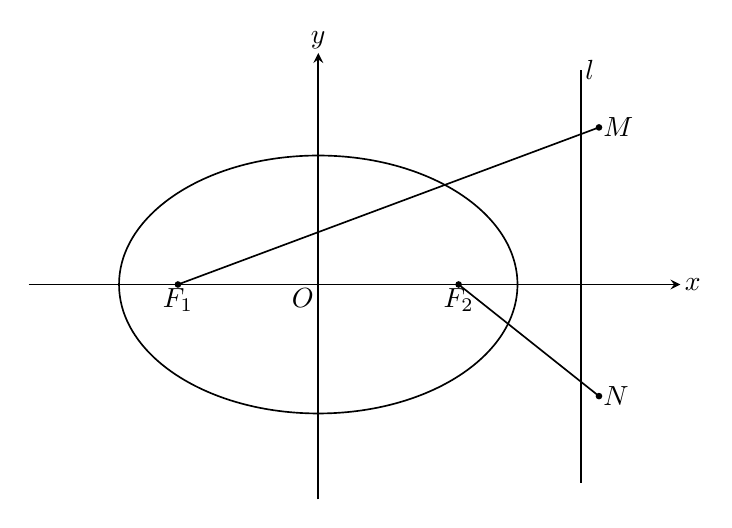
\begin{tikzpicture}[x=1.15cm, y=1.05cm, semithick, every node/.style={inner sep=1.3pt}]
  \draw[->,>=stealth] (-3.2,0) -- (4.0,0) node[right] {$x$};
  \draw[->,>=stealth] (0,-2.6) -- (0,2.8) node[above] {$y$};
  \node[below left] at (0,0) {$O$};

  \draw (0,0) ellipse [x radius=2.2, y radius=1.56];

  \coordinate (F1) at (-1.55,0);
  \coordinate (F2) at (1.55,0);
  \coordinate (M) at (3.1,1.9);
  \coordinate (N) at (3.1,-1.35);

  \draw (2.9,-2.4) -- (2.9,2.6);
  \node[right] at (2.9,2.6) {$l$};

  \draw (F1) -- (M);
  \draw (F2) -- (N);

  \fill (F1) circle (1.2pt); \node[below] at (F1) {$F_1$};
  \fill (F2) circle (1.2pt); \node[below] at (F2) {$F_2$};
  \fill (M) circle (1.2pt); \node[right] at (M) {$M$};
  \fill (N) circle (1.2pt); \node[right] at (N) {$N$};
\end{tikzpicture}
\end{center}
\nopagebreak[4]
\Needspace{4\baselineskip}
\textbf{解析}

\Needspace{5\baselineskip}
由 $e=\dfrac{\sqrt2}2$ 得 $c=\dfrac a{\sqrt2}$，右准线 $l:x=a\sqrt2$。设 $M(a\sqrt2,m)$、$N(a\sqrt2,n)$，则

\nopagebreak[4]
\[\overrightarrow{F_1M}=\left(\frac{3a}{\sqrt2},m\right),\qquad \overrightarrow{F_2N}=\left(\frac a{\sqrt2},n\right),\]

条件 $\overrightarrow{F_1M}\cdot\overrightarrow{F_2N}=0$ 给出 $\dfrac{3a^2}2+mn=0$，即 $mn=-\dfrac{3a^2}2$。

\Needspace{5\baselineskip}
（1）由 $\left|\overrightarrow{F_1M}\right|=\left|\overrightarrow{F_2N}\right|=2\sqrt5$：

\nopagebreak[4]
\[\frac{9a^2}2+m^2=20,\qquad \frac{a^2}2+n^2=20.\]

\Needspace{5\baselineskip}
两式相乘并代入 $m^2n^2=\dfrac{9a^4}4$，得

\nopagebreak[4]
\[\left(20-\frac{9a^2}2\right)\left(20-\frac{a^2}2\right)=\frac{9a^4}4\iff 400-100a^2=0,\]

故 $a^2=4$，$a=2$，$c=\sqrt2$，$b^2=a^2-c^2=2$，即 $b=\sqrt2$。

\Needspace{5\baselineskip}
（2）

\nopagebreak[4]
\[|MN|=|m-n|=|m|+|n|\geqslant2\sqrt{|mn|}=a\sqrt6,\]

\Needspace{5\baselineskip}
等号当 $|m|=|n|=a\sqrt{\dfrac32}$ 时成立，此时 $m+n=0$，于是

\nopagebreak[4]
\[\overrightarrow{F_1M}+\overrightarrow{F_2N}=\left(2\sqrt2a,\ m+n\right)=(2\sqrt2a,0)\parallel\overrightarrow{F_1F_2},\]

即 $|MN|$ 最小时 $\overrightarrow{F_1M}+\overrightarrow{F_2N}$ 与 $\overrightarrow{F_1F_2}$ 共线。

\gkanswer{答案：（1）$a=2$，$b=\sqrt2$；（2）证明见解析。}

\end{answer}
\begin{answer}
\gksolhead{22}{}

\textbf{题目}：

已知 $x=3$ 是函数 $f(x)=a\ln(1+x)+x^2-10x$ 的一个极值点。

（1）求 $a$；

（2）求函数 $f(x)$ 的单调区间；

（3）若直线 $y=b$ 与函数 $y=f(x)$ 的图象有 $3$ 个交点，求 $b$ 的取值范围。

\Needspace{4\baselineskip}
\textbf{解析}

（1）$f'(x)=\dfrac a{1+x}+2x-10$，由 $f'(3)=\dfrac a4-4=0$ 得 $a=16$。

（2）此时 $f'(x)=\dfrac{16+2x^2-8x}{1+x}=\dfrac{2(x-1)(x-3)}{1+x}$（$x>-1$），故 $f$ 在 $(-1,1)$ 上递增、$(1,3)$ 上递减、$(3,+\infty)$ 上递增。

\Needspace{5\baselineskip}
（3）$f(1)=16\ln2-9$（极大值），$f(3)=16\ln4-21=32\ln2-21$（极小值）；又 $x\to-1^+$ 时 $f\to-\infty$，$x\to+\infty$ 时 $f\to+\infty$。直线 $y=b$ 与图象有三个交点当且仅当

\nopagebreak[4]
\[32\ln2-21<b<16\ln2-9.\]

\gkanswer{答案：（1）$a=16$；（2）增区间 $(-1,1)$、$(3,+\infty)$，减区间 $(1,3)$；（3）$\left(32\ln2-21,\ 16\ln2-9\right)$。}

\end{answer}